\documentclass{beamer}
\usetheme{tokitex}

\usepackage{graphics}
\usepackage{multirow}
\usepackage{tabto}

\usepackage[english,bahasa]{babel}
\newtranslation[to=bahasa]{Section}{Bagian}
\newtranslation[to=bahasa]{Subsection}{Subbagian}

\usepackage{listings, lstautogobble}
\usepackage{color}

\definecolor{dkgreen}{rgb}{0,0.6,0}
\definecolor{gray}{rgb}{0.5,0.5,0.5}
\definecolor{mauve}{rgb}{0.58,0,0.82}

\lstset{frame=tb,
  language=pascal,
  aboveskip=1mm,
  belowskip=1mm,
  showstringspaces=false,
  columns=fullflexible,
  keepspaces=true,
  basicstyle={\small\ttfamily},
  numbers=none,
  numberstyle=\tiny\color{gray},
  keywordstyle=\color{blue},
  commentstyle=\color{dkgreen},
  stringstyle=\color{mauve},
  breaklines=true,
  breakatwhitespace=true,
  autogobble=true
}

\title{Dynamic Programming: \newline Studi Kasus}
\author{Tim Olimpiade Komputer Indonesia}
\date{}

\usepackage{qtree}
\begin{document}

\begin{frame}
\titlepage
\end{frame}

\begin{frame}
\frametitle{Pendahuluan}
Melalui dokumen ini, kalian akan:
\begin{itemize}
  \item Menyelesaikan beberapa contoh persoalan DP sederhana.
  \item Membiasakan diri untuk "berpikir secara DP".
\end{itemize}
\end{frame}

\begin{frame} 
\frametitle{Contoh Soal 1: Knapsack}
\begin{itemize}
  \item Diberikan $N$ buah barang. 
  \item Barang ke-$i$ memiliki harga $v_i$ rupiah dan berat $w_i$ gram. 
  \item Kita memiliki tas yang berkapasitas $G$ gram. 
  \item Kita ingin memasukan beberapa barang kedalam tas, sedemikian sehingga jumlah berat dari barang-barang yang kita masukan tidak lebih dari kapasitas tas dan jumlah harganya sebanyak mungkin.
\end{itemize}
\end{frame}

\begin{frame} 
\frametitle{Observasi}
\begin{itemize}
  \item Untuk setiap barang, kita harus memutuskan apakah barang ini diambil atau tidak.
  \item Jika diambil, kapasitas tas kita berkurang, dan harga barang yang kita dapatkan bertambah.
  \item Jika tidak diambil, tidak terjadi perubahan.
\end{itemize}
\end{frame}

\begin{frame} 
\frametitle{Formulasi}
\begin{itemize}
  \item Definisikan sebuah fungsi $g(x,y)$ sebagai jumlah harga maksimum yang mungkin diperoleh, jika kita hanya mempunyai barang ke-$1$ sampai ke-$x$ dan kapasitas tas kita adalah $y$ gram.
  \item Untuk menghitung fungsi $g(x,y)$ kita bisa mencoba-coba apakah kita akan memasukan barang ke-$x$ ke tas atau tidak.
\end{itemize}
\end{frame}

\begin{frame} 
\frametitle{Formulasi Rekurens}
\begin{itemize}
  \item Jika kita memasukan barang ke-$x$ ke tas, maka kita akan menyisakan barang ke-$1$ sampai ke-$(x-1)$ dan sisa kapasitas tas adalah $y-w_x$. 
  \item Harga barang yang didapatkan pada kasus ini adalah $g(x-1,y-w_x)$ ditambah dengan harga yang kita peroleh pada barang ke-$x$.
  \item Dapat dituliskan $g(x, y) = g(x-1, y-w_x) + v_x$.
  \item Kasus ini hanya boleh dipertimbangkan jika $y \geq w_x$.
\end{itemize}
\end{frame}

\begin{frame} 
\frametitle{Formulasi Rekurens (lanj.)}
\begin{itemize}
  \item Jika kita tidak memasukan barang ke-$x$ ke tas, maka kita akan menyisakan barang ke-$1$ sampai ke-$(x-1)$ dan sisa kapasitas tas masih tetap $y$.
  \item Harga barang didapatkan pada kasus ini adalah $g(x-1,y)$, tanpa tambahan apapun (kita tidak mengambil barang ke-$x$).
  \item Dapat dituliskan $g(x, y) = g(x-1, y)$.
\end{itemize}
\end{frame}

\begin{frame} 
\frametitle{Formulasi Rekurens (lanj.)}
\begin{itemize}
  \item Dari kedua pilihan keputusan tersebut, kita tertarik dengan yang menghasilkan nilai terbesar.
  \item Cukup bandingkan mana yang lebih besar, antara:
  \begin{itemize}
    \item $g(x-1, y-w_x) + v_x$, atau
    \item $g(x-1, y)$
  \end{itemize}
  \item Dapat dituliskan: $g(x, y) = \max(g(x-1,y-w_x)+v_x,g(x-1,y))$. \newline
  \item Kembali ditekankan bahwa pilihan memasukkan barang ke-$x$ hanya boleh dipertimbangkan jika $y \geq w_x$.
\end{itemize}
\end{frame}

\begin{frame} 
\frametitle{Formulasi Base Case}
\begin{itemize}
  \item Jika $x=0$, maka berarti tidak ada lagi barang yang tersedia. 
  \item Ini berarti $g(x,y) = 0$.
  \item Kasus ini menjadi \fbasecase.
\end{itemize}
\end{frame}

\begin{frame} 
\frametitle{Formulasi Akhir}
$g(x,y)$ dapat dirumuskan sebagai berikut:
\begin{small}
\[g(x,y) = \left\{\begin{array}{lr}
    0, & x = 0\\
    g(x-1,y), & x > 0 \wedge y < w_x\\
    \max(g(x-1,y-w_x)+v_x,g(x-1,y)), & x > 0 \wedge y \geq w_x\\
    \end{array}\right.\]
\end{small}
\end{frame}

\begin{frame} 
\frametitle{Analisis Kompleksitas}
\begin{itemize}
  \item Terdapat $O(N)$ nilai berbeda untuk nilai $x$ dan $O(G)$ nilai berbeda untuk nilai $y$ pada $g(x,y)$.
  \item Dibutuhkan $O(1)$ untuk menghitung $g(x,y)$. 
  \item Sehingga untuk menghitung seluruh nilai $g(x,y)$ untuk seluruh $x$ dan $y$ dibutuhkan waktu $O(NG)$.
\end{itemize}
\end{frame}

\begin{frame}
\frametitle{Solusi Top Down}
Kita implementasikan $g(x, y)$ sebagai fungsi $\proc{solve}(x,y)$:
\begin{codebox}
\Procname{$\proc{solve}(x, y)$}
\li \If $(x \isequal 0)$ \Then
\li   \Return $0$
\li \ElseIf $hasComputed[x][y]$ \Then
\li   \Return $memo[x][y]$ 
\li \Else
\li   $best \gets \proc{solve}(x-1, y)$
\li   \If $(y \geq w[x])$ \Then
\li     $best \gets \max(best, \proc{solve}(x - 1, y-w[x]) + v[x])$
      \End  
\li   $hasComputed[x][y] \gets true$
\li   $memo[x][y] \gets best$
\li   \Return $best$
    \End
\end{codebox}

Jawaban ada pada $\proc{solve}(N, G)$
\end{frame}

\begin{frame}
\frametitle{Solusi Bottom Up}
\begin{codebox}
\Procname{$\proc{solve}()$}
\li \For $y \gets 0$ \To $G$ \Do
\li   $g[0][y] \gets 0$ \Comment Base case...
    \End
\zi
\li \Comment Isi "tabel" dari kasus yang kecil ke besar
\li \For $x \gets 1$ \To $N$ \Do
\li   \For $y \gets 0$ \To $G$ \Do
\li     $best \gets g[x-1][y]$
\li     \If $(y \geq w[x])$ \Then
\li       $best \gets \max(best, g[x - 1][y-w[x]] + v[x])$
        \End  
\li     $g[x][y] \gets best$
      \End
    \End    
\li \Return $g[N][G]$
    \End
\end{codebox}
\end{frame}

\begin{frame}
\frametitle{Contoh Soal 2: Memotong Kayu}
\begin{itemize}
  \item Kita akan memotong sebuah batang kayu dengan panjang $M$ meter pada $N$ titik menjadi $N+1$ bagian.
  \item Titik ke-$i$ berada di $L_i$ meter dari ujung kiri.
  \item Untuk memotong sebatang kayu menjadi dua, kita memerlukan usaha \alert{sebesar panjang kayu yang sedang kita potong}.
  \item Cari urutan pemotongan sedemikian sehingga total usaha yang dibutuhkan minimum!
\end{itemize}
\end{frame}

\begin{frame}
\frametitle{Contoh Soal 2: Memotong Kayu (lanj.)}
Sebagai contoh, terdapat sebuah kayu dengan panjang 10 meter dan terdapat 3 titik potongan pada 2 meter, 4 meter, dan 7 meter dari ujung kiri.
\begin{figure}
  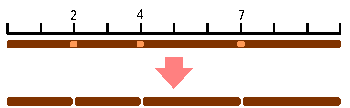
\includegraphics[width=10cm]{asset/cutting-stick-1.pdf}
\end{figure}
\end{frame}

\begin{frame}
\frametitle{Contoh Soal 2: Memotong Kayu (lanj.)}
Kita bisa memotong pada titik 2, titik 4, lalu titik 7 dan memerlukan usaha 10 + 8 + 6 = 24.
\begin{figure}
  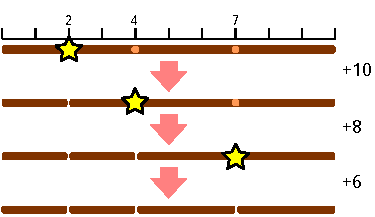
\includegraphics[width=10cm]{asset/cutting-stick-2.pdf}
\end{figure}
\end{frame}

\begin{frame}
\frametitle{Contoh Soal 2: Memotong Kayu (lanj.)}
Cara lain adalah memotong pada titik 4, titik 2, lalu titik 7 dan memerlukan usaha 10 + 4 + 6 = 20.
\begin{figure}
  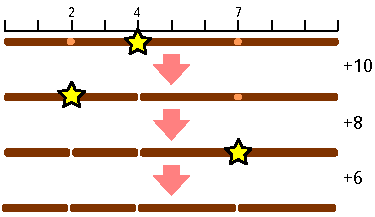
\includegraphics[width=10cm]{asset/cutting-stick-3.pdf}
\end{figure}
\end{frame}

\begin{frame}
\frametitle{Solusi Greedy?}
\begin{itemize}
  \item Apakah strategi \fGreedy dengan memotong "setengah-tengahnya" selalu menghasilkan solusi optimal?
  \item Bagaimana dengan kasus jika $M = 2000$ dan $L = [1, 2, 3, 4, 5, 1000]$?
  \item Kita akan coba menggunakan DP untuk persoalan ini.
\end{itemize}
\end{frame}

\begin{frame}
\frametitle{Observasi}
\begin{itemize}
  \item Untuk pemotongan pertama, terdapat $N$ pilihan lokasi pemotongan.
  \item Jika kita memotong di posisi $L_x$, maka didapatkan dua batang.
  \item Batang pertama perlu dipotong di titik $L_1, L_2, ..., L_{x-1}$ dan batang kedua di $L_{x+1}, L_{x+2}, ..., L_N$.
  \item Ternyata kita mendapatkan sub-persoalan yang serupa.
  \item Pemotongan bisa dilanjutkan secara rekursif, dan kita pilih posisi pemotongan yang ke depannya membutuhkan usaha terkecil.
\end{itemize}
\end{frame}

\begin{frame}
\frametitle{Formulasi Rekurens}
\begin{itemize}
  \item Definisikan sebuah fungsi $g(x,y)$ sebagai jumlah usaha minimum yang mungkin diperoleh, jika kita hanya perlu memotong di $L_{x}, L_{x+1}, ..., L_{y}$.
  \item Untuk menghitung $g(x,y)$ kita dapat mencoba titik mana yang kita potong pertama kali.
  \item Jika kita memotong di $L_k$ $(x \leq k \leq y)$, maka kita akan mendapatkan dua potongan.
\end{itemize}
\begin{figure}
  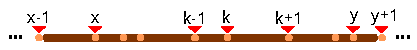
\includegraphics[width=10cm]{asset/cutting-stick-4.pdf}
\end{figure}
\end{frame}

\begin{frame}
\frametitle{Formulasi Rekurens (lanj.)}
\begin{figure}
  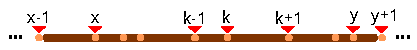
\includegraphics[width=10cm]{asset/cutting-stick-4.pdf}
\end{figure}
\begin{itemize}
  \item Total usaha yang dibutuhkan jika kita melakukan pemotongan di $L_k$ adalah jumlah dari:
  \begin{itemize}
    \item Total usaha minimum dari potongan pertama, yaitu $g(x,k-1)$.
    \item Total usaha minimum dari potongan kedua, yaitu $g(k+1,y)$.
    \item Usaha untuk pemotongan ini, yaitu $L_{y+1} - L_{x-1}$.
  \end{itemize}
  \item Untuk mempermudah, asumsikan $L_0 = 0$ dan $L_{N+1} = M$.
\end{itemize}
\end{frame}

\begin{frame} 
\frametitle{Formulasi Base Case}
\begin{itemize}
  \item Ketika $x>y$, artinya sudah tidak ada pemotongan yang perlu dilakukan.
  \item Dengan demikian, usaha yang dibutuhkan adalah 0, atau $g(x,y) = 0$.
\end{itemize}
\end{frame}

\begin{frame} 
\frametitle{Formulasi Akhir}
Dapat dirumuskan:
\begin{small}
\[g(x,y) = \left\{\begin{array}{lr}
    0, & x>y\\
    \min_{x \leq k \leq y} g(x,k-1) + g(k+1,y) + (L_{y+1} - L_{x-1}), & x \leq y \\
    \end{array}\right.\]
\end{small}
\end{frame}

\begin{frame} 
\frametitle{Analisis Kompleksitas}
\begin{itemize}
  \item Terdapat $O(N)$ nilai berbeda untuk nilai $x$ dan $O(N)$ nilai berbeda untuk nilai $y$ pada $g(x,y)$.
  \item Dibutuhkan iterasi sebanyak $O(N)$ untuk menghitung $g(x,y)$. 
  \item Sehingga untuk menghitung seluruh nilai $g(x,y)$ untuk seluruh $x$ dan $y$ dibutuhkan waktu $O(N^3)$.
\end{itemize}
\end{frame}

\begin{frame}
\frametitle{Solusi Top Down}
Kita implementasikan $g(x, y)$ sebagai fungsi $\proc{solve}(x,y)$:
\begin{small}
\begin{codebox}
\Procname{$\proc{solve}(x, y)$}
\li \If $(x > y)$ \Then
\li   \Return $0$
\li \ElseIf $hasComputed[x][y]$ \Then
\li   \Return $memo[x][y]$ 
\li \Else
\li   $best \gets \infty$
\li   $cost \gets L[y+1] - L[x-1]$
\li   \For $k \gets x$ \To $y$ \Do
\li     $best \gets \min(best, \proc{solve}(x,k-1) + \proc{solve}(k+1, y) + cost)$
      \End  
\li   $hasComputed[x][y] \gets true$
\li   $memo[x][y] \gets best$
\li   \Return $best$
    \End
\end{codebox}
\end{small}
Jawaban ada pada $\proc{solve}(1, N)$
\end{frame}

\begin{frame}
\frametitle{Solusi Bottom Up}
\begin{small}
\begin{codebox}
\Procname{$\proc{solve}()$}
\li \Comment Inisialisasi base case
\li \For $x \gets 0$ \To $N+1$ \Do
\li   \For $y \gets 0$ \To $x-1$ \Do
\li     $g[x][y] \gets 0$
      \End
    \End
\zi
\li \Comment Isi "tabel" mulai dari kasus yang kecil
\li \For $gap \gets 0$ \To $N$ \Do
\li   \For $x \gets 1$ \To $N-gap$ \Do
\li     $y \gets x + gap$
\li     $best \gets \infty$
\li     $cost \gets L[y+1] - L[x-1]$
\li     \For $k \gets x$ \To $y$ \Do
\li       $best \gets \min(best, g[x][k-1] + g[k+1][y] + cost)$
        \End  
\li     $g[x][y] \gets best$
      \End
    \End
\zi
\li \Return $g[1][N]$
\end{codebox}
\end{small}
\end{frame}

\begin{frame}
\frametitle{Pengisian "Tabel" DP}
\begin{itemize}
  \item Perhatikan bahwa pada metode \fbottomup, pengisian "tabel" dilakukan secara "tidak biasa".
  \item Kita perlu mengisi mulai dari:
  \begin{itemize}
    \item $g[1][1], g[2][2], ..., g[N][N]$,
    \item lalu $g[1][2], g[2][3], ..., g[N-1][N]$,
    \item lalu $g[1][3], g[2][4], ..., g[N-2][N]$,
    \item lalu $g[1][4], g[2][5], ..., g[N-3][N]$,    
    \item dan seterusnya sampai $g[1][N]$.
  \end{itemize}
  \item Ingat bahwa pengisian "tabel" harus dilakukan dari kasus yang kecil ke besar.
  \item Definisi "kasus kecil" pada masalah ini adalah kayu dengan titik-titik pemotongan yang lebih sedikit.
\end{itemize}
\end{frame}

\begin{frame}
\frametitle{Pengisian "Tabel" DP (lanj.)}
\begin{itemize}
  \item Dari contoh ini kita mempelajari bahwa urutan pengisian "tabel" pada DP \fbottomup tidak selalu biasa.
  \item Jika urutan pengisiannya salah, maka hasil akhir yang didapatkan juga bisa jadi salah.
  \item Hal in terjadi ketika kita hendak menyelesaikan kasus yang besar, tetapi hasil untuk kasus-kasus yang lebih kecil belum tersedia.
  \item Untuk mengetahui urutan pengisian "tabel", Anda perlu mengamati apa definisi "kasus kecil" pada masalah yang dihadapi.
\end{itemize}
\end{frame}

\begin{frame}
\frametitle{Penutup}
\begin{itemize}
  \item DP merupakan topik yang cukup luas untuk dibicarakan.
  \item Banyak berlatih mengerjakan soal DP dapat melatih kita untuk mendapatkan rumus DP yang sesuai dengan masalah yang dihadapi.
  \item Topik optimisasi lainnya pada DP akan dibahas pada kesempatan yang lain.  
\end{itemize}
\end{frame}

\end{document}
